\documentclass[12pt,aspectratio=169]{beamer}

% ====================================================
% ====================================================
% USEPACKAGES AND IMPORTS
% ====================================================
% ====================================================

\usepackage[T1]{fontenc}
\usepackage[utf8]{inputenc}
\usepackage[english]{babel}

% tables
\usepackage{tabularx}
\usepackage{colortbl}
\usepackage{multirow}
\usepackage{makecell}

% tikz and colors
\usepackage{tikz}
\usepackage{xcolor}
\usepackage{pgfplots}
\usepackage{pgfplotstable}
\usepackage{tikzsymbols}

\usetikzlibrary{calc}
\usetikzlibrary{trees}
\usetikzlibrary{patterns}
\usetikzlibrary{shadings}
\usetikzlibrary{positioning}
\usetikzlibrary{intersections}
\usepgfplotslibrary{patchplots}
\usepgfplotslibrary{fillbetween}
\usetikzlibrary{decorations.pathreplacing}

\usetikzlibrary{arrows}
\usetikzlibrary{arrows.meta}

\usetikzlibrary{shapes}
\usetikzlibrary{shapes.arrows}
\usetikzlibrary{shapes.callouts}
\usetikzlibrary{shapes.symbols}
\usetikzlibrary{shapes.geometric}

% boxes
\usepackage[many]{tcolorbox}

% math packages and fonts
\usepackage{bm}
\usepackage{ccfonts}
\usepackage{eulervm}
\usepackage{amsmath}
\usepackage{amsfonts}
\usepackage{amssymb}
\usepackage{amsthm}
\usepackage{mathtools}
\usepackage{nicefrac}
\usepackage{slashed}
\usepackage{bbold}
\usepackage{array}
\usepackage{cancel}

% algorithms and listings
\usepackage[ruled,vlined,linesnumbered]{algorithm2e}
\usepackage{listings}
\usepackage{setspace}

\tcbuselibrary{listings}
\tcbuselibrary{breakable}
\tcbuselibrary{skins}

% misc
\usepackage{soul}
\usepackage{pifont}
\usepackage{skull}
\usepackage{multicol}
\usepackage{animate}
\usepackage{hyperref}
\usepackage{wasysym}
\usepackage[absolute,overlay]{textpos}
\usepackage[hang,flushmargin]{footmisc}

% ====================================================
% ====================================================
% LAYOUT AND THEME
% ====================================================
% ====================================================

\usetheme{Copenhagen}

% color definitions
\definecolor{myblue1}{RGB}{35,119,189}
\definecolor{myblue2}{RGB}{95,179,238}
\definecolor{myblue3}{RGB}{129,168,207}
\definecolor{myblue4}{RGB}{26,89,142}

\definecolor{myred1}{RGB}{247,12,12}

% set theme colors
\setbeamercolor*{structure}{fg=myblue1,bg=blue}
\setbeamercolor*{palette primary}{use=structure,fg=white,bg=structure.fg}
\setbeamercolor*{palette secondary}{use=structure,fg=white,bg=structure.fg!75!black}
\setbeamercolor*{palette tertiary}{use=structure,fg=white,bg=structure.fg!50!black}
\setbeamercolor*{palette quaternary}{fg=black,bg=white}

\setbeamertemplate{itemize item}[circle]
\setbeamertemplate{itemize subitem}[circle]
\setbeamertemplate{itemize subsubitem}[circle]

\setbeamertemplate{enumerate item}[circle]
\setbeamertemplate{enumerate subitem}[circle]
\setbeamertemplate{enumerate subsubitem}[circle]

\setbeamercolor{itemize item}{fg=myblue1}
\setbeamercolor{itemize subitem}{fg=myblue1}
\setbeamercolor{itemize subsubitem}{fg=myblue1}

\setbeamertemplate{section in toc}[circle]
\setbeamertemplate{subsection in toc}[circle]
\setbeamerfont{subsection in toc}{size=\scriptsize}

\setbeamercolor{frametitle continuation}{fg=black}

% title graphic -- sap logo and dhbw logo
\titlegraphic{
\includegraphics[scale=0.1]{../03_img/logo_sap}\hspace*{4.75cm}~%
   	
\includegraphics[scale=0.05]{../03_img/logo_dhbw}
}

\makeatletter
% frame title
\defbeamertemplate*{frametitle}{mydefault}[1][left]
{
  	\ifbeamercolorempty[bg]{frametitle}{}{\nointerlineskip}%
  	\nointerlineskip%
 	\@tempdima=\textwidth%
  	\advance\@tempdima by\beamer@leftmargin%
  	\advance\@tempdima by\beamer@rightmargin%
  	\begin{tcolorbox}[
  		enhanced,
  		outer arc=0pt,
  		arc=0pt,
  		boxrule=0pt,
  		top=0pt,
  		bottom=0pt,
  		enlarge left by=-\beamer@leftmargin,
  		enlarge right by=-\beamer@rightmargin,
  		width=\paperwidth,
  		nobeforeafter,
  		interior style={
    			left color=myblue2,
    			right color=white
    		},
  		shadow={0mm}{-0.4mm}{0mm}{black!60,opacity=0.6},    
  		shadow={0mm}{-0.8mm}{0mm}{black!40,opacity=0.4},    
  	]
    	\usebeamerfont{frametitle}%
    	\vbox{}\vskip-1ex%
    	\if@tempswa\else\csname beamer@fte#1\endcsname\fi%
    	\insertframetitle\par%
    	{%
      		\ifx\insertframesubtitle\@empty%
      		\else%
      		{\usebeamerfont{framesubtitle}\usebeamercolor[fg]{black}\insertframesubtitle\strut\par}%
      		\fi
    	}%
    	\vskip-1ex%
    	\if@tempswa\else\vskip-.3cm\fi
  	\end{tcolorbox}%
}

% footline of a frame
\defbeamertemplate*{footline}{mysplit theme}
{%
  	\leavevmode%
  	\hbox{
		\begin{beamercolorbox}[
			wd=.5\paperwidth,ht=2.5ex,dp=1.125ex,leftskip=.3cm plus1fill,rightskip=.3cm
		]{author in head/foot}%
    			\usebeamerfont{author in head/foot}\insertshortauthor\ (\insertinstitute), \insertdate
  		\end{beamercolorbox}%
  		\begin{beamercolorbox}[
			wd=.5\paperwidth,ht=2.5ex,dp=1.125ex,leftskip=.3cm,rightskip=.3cm plus1fil
		]{title in head/foot}%
    			\usebeamerfont{title in head/foot}\insertshorttitle\hfill
    			\insertprefix-\insertframenumber/\inserttotalframenumber\hspace*{0.5em}
  		\end{beamercolorbox}}%
  	\vskip0pt%
}
\makeatother

% ====================================================
% ====================================================
% COMMANDS AND GENERAL DEFINITIONS
% ====================================================
% ====================================================

% page number prefix
\newcommand\insertprefix{}  % empty by default
\newcommand\prefix[1]{\renewcommand\insertprefix{#1}}

% math definitions
% ====================================================
\DeclareMathOperator*{\argmax}{arg\,max}
\DeclareMathOperator*{\argmin}{arg\,min}
\newcommand*\diff{\mathop{}\!\mathrm{d}}

\newcommand*{\vertbar}{\rule[-1ex]{0.5pt}{2.5ex}}
\newcommand*{\horzbar}{\rule[.5ex]{2.5ex}{0.5pt}}

% commands
% ====================================================

% highlight commands
% --------------------------------------------------------------------------------------------------------
% highlight command
\newcommand{\highlight}[1]{\textcolor{myblue1}{\textbf{#1}}}
\newcommand{\highlighttt}[1]{\textcolor{myblue1}{\texttt{#1}}}
\newcommand{\Highlight}[1]{\textcolor{myred1}{\textbf{#1}}}

% blue color boxes (with frame/without frame/without fill)
\newtcolorbox{boxBlue}{colback=myblue1!10!white,colframe=myblue4}
\newtcolorbox{boxBlueNoFrame}{colback=myblue1!10!white,colframe=myblue1!10!white}
\newtcolorbox{boxBlueNoFill}{colback=white,colframe=myblue4}

% font commands
% --------------------------------------------------------------------------------------------------------
\newcommand{\linkstyle}[1]{\underline{\smash{\texttt{#1}}}} 		% style of hyperlinks

% tikz commands
% --------------------------------------------------------------------------------------------------------

% yellow sticky note
\newcommand{\bubble}[3]{
\begin{textblock}{100}(#1, #2)
      	\begin{tikzpicture}
		\node[rectangle,draw=yellow,very thick,fill=yellow!60,align=center] at (0,0) {#3};
	\end{tikzpicture}
\end{textblock}
}

\newcommand{\floattext}[3]{
\begin{textblock}{100}(#1, #2)
      	#3
\end{textblock}
}

\newcommand{\doublecircle}[2]{
	\draw[fill=white,draw=myblue1] (#1,#2) circle (2mm);
	\draw[fill=myblue1,draw=myblue1] (#1,#2) circle (1.5mm);
}

% slide modifiers
% --------------------------------------------------------------------------------------------------------
% mark slide as optional
\newcommand{\optional}{
	\begin{textblock}{100}(0.15,0.30)
      		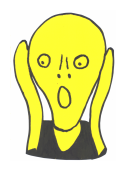
\includegraphics[scale=0.2]{../03_img/scream}
    	\end{textblock}
}

% mark slide as important
\newcommand{\important}{
	\begin{textblock}{100}(0.10,0.15)
      		
\includegraphics[scale=0.1]{../03_img/important}
    	\end{textblock}
}

% citation
% --------------------------------------------------------------------------------------------------------
% first argument in {book, online, article}
\newcommand{\literature}[5]{
	\setbeamertemplate{bibliography item}[#1]
	\bibitem{#2}
	\highlight{#3} \\
	\textcolor{darkgray}{\textit{#4}} \\
	\textcolor{black}{#5}
}
% cite content
\newcommand{\citeAuthor}[3]{\vfill\scriptsize\textcolor{lightgray}{#1 \cite{#2} #3}}

% slide architecture
% --------------------------------------------------------------------------------------------------------
% divide frame into two parts
\newcommand{\divideTwo}[4]{
	\begin{minipage}{#1\textwidth}
		#2
	\end{minipage}
	\hfill
	\begin{minipage}{#3\textwidth}
		#4
	\end{minipage}
}

% divide frame into two parts (start on top)
\newcommand{\divideTwoTop}[4]{
	\begin{minipage}[t]{#1\textwidth}
		#2
	\end{minipage}
	\hfill
	\begin{minipage}[t]{#3\textwidth}
		#4
	\end{minipage}
}

% special pages
% --------------------------------------------------------------------------------------------------------
% title page
\newcommand{\maketitlepage}{
	{
		\beamertemplatenavigationsymbolsempty
		\usebackgroundtemplate{%
			\tikz[overlay,remember picture] \node[opacity=0.2, at=(current page.center)] {
  				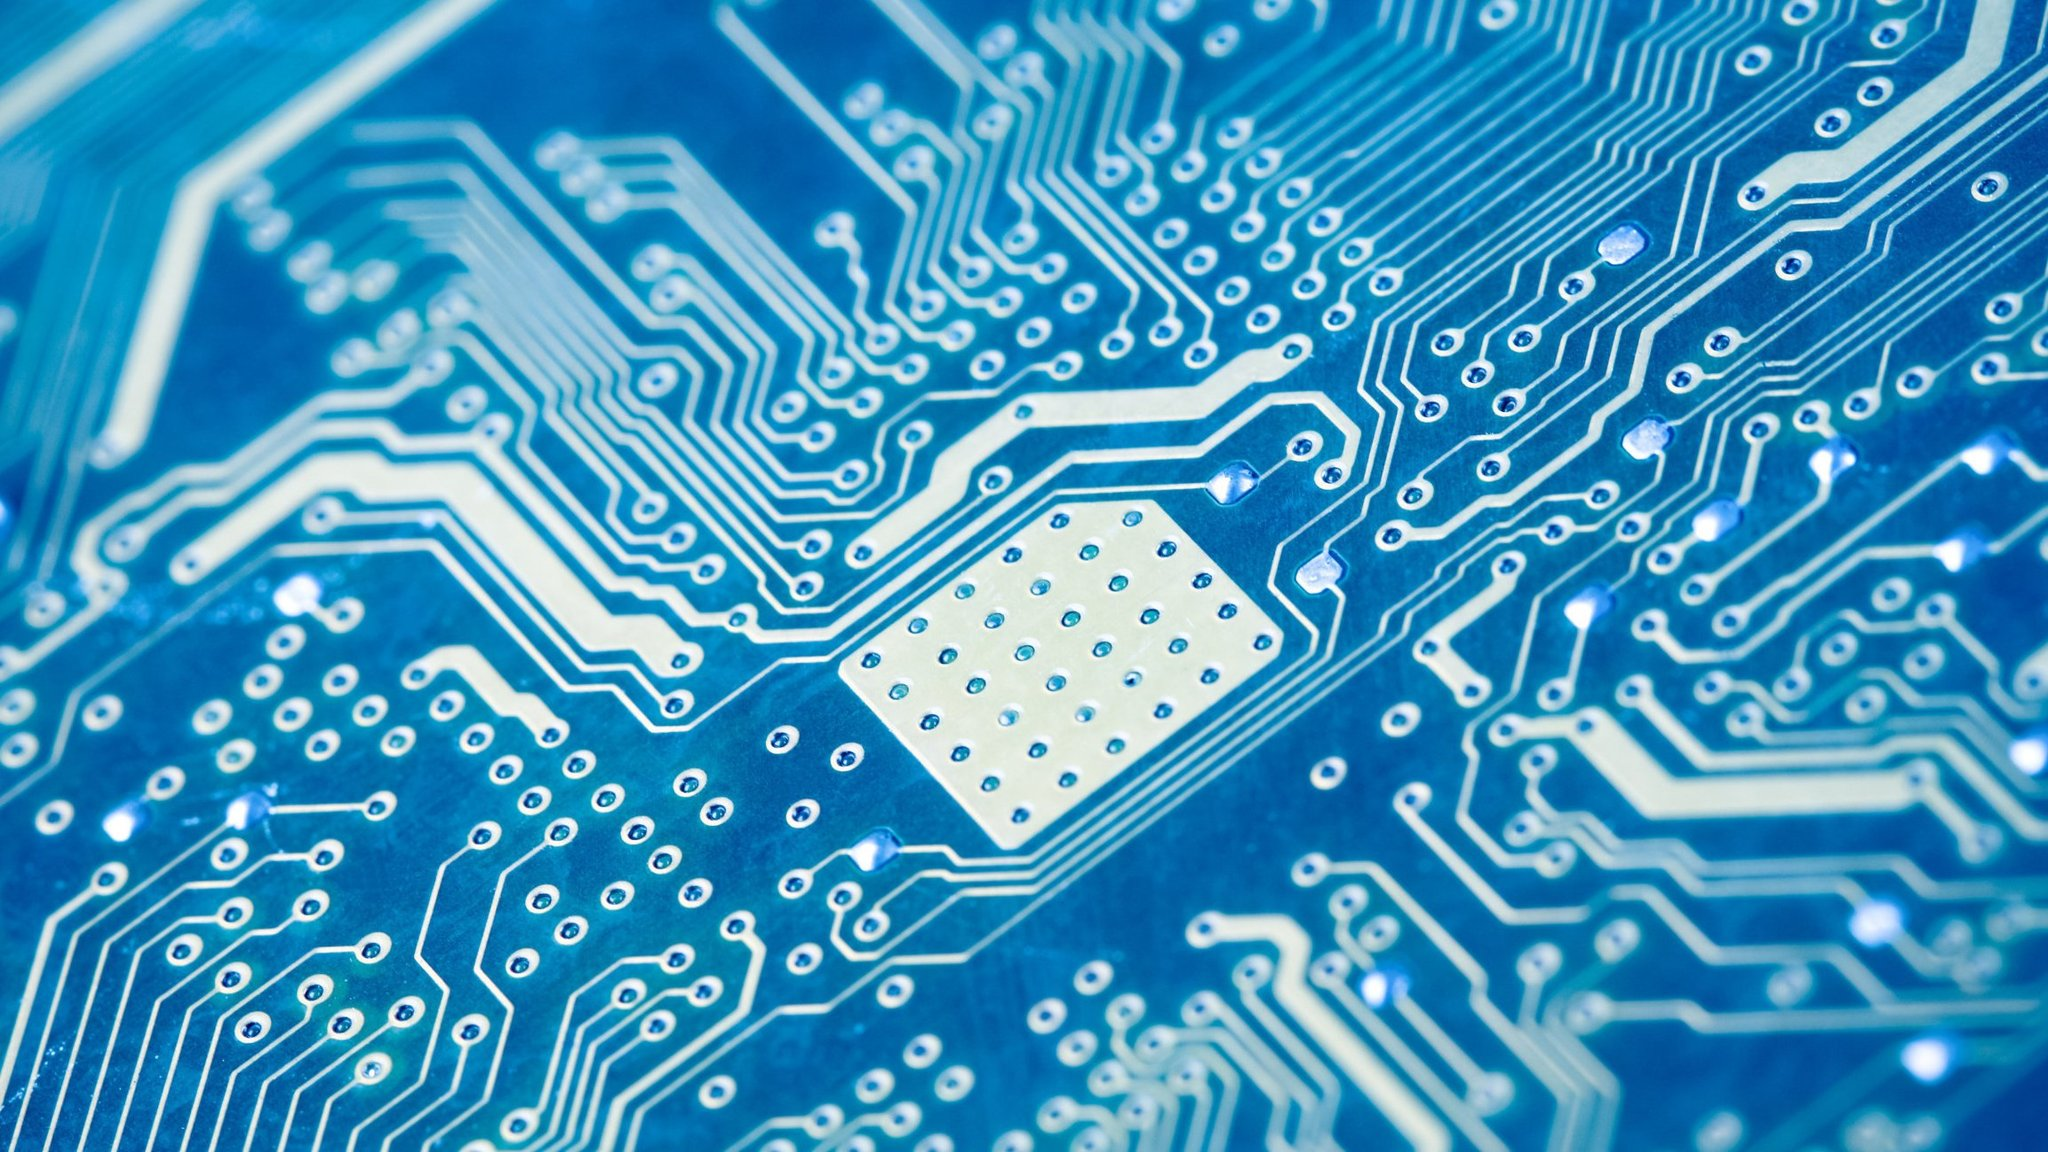
\includegraphics[height=\paperheight,width=\paperwidth]{../03_img/processor.jpg}
			};
		}
		\begin{frame}[plain]
			\vspace*{0.75cm}
			\maketitle
			\vfill
			\begin{center}
				\footnotesize Find all slides on \href{https://github.com/DaWe1992/Applied_ML_Fundamentals}{\linkstyle{GitHub}}
			\end{center}
		\end{frame}
	}
}

% divider page
\newcommand{\makedivider}[1]{
	{
		\beamertemplatenavigationsymbolsempty
		\usebackgroundtemplate{%
			\tikz[overlay,remember picture] \node[opacity=0.2, at=(current page.center)] {
  				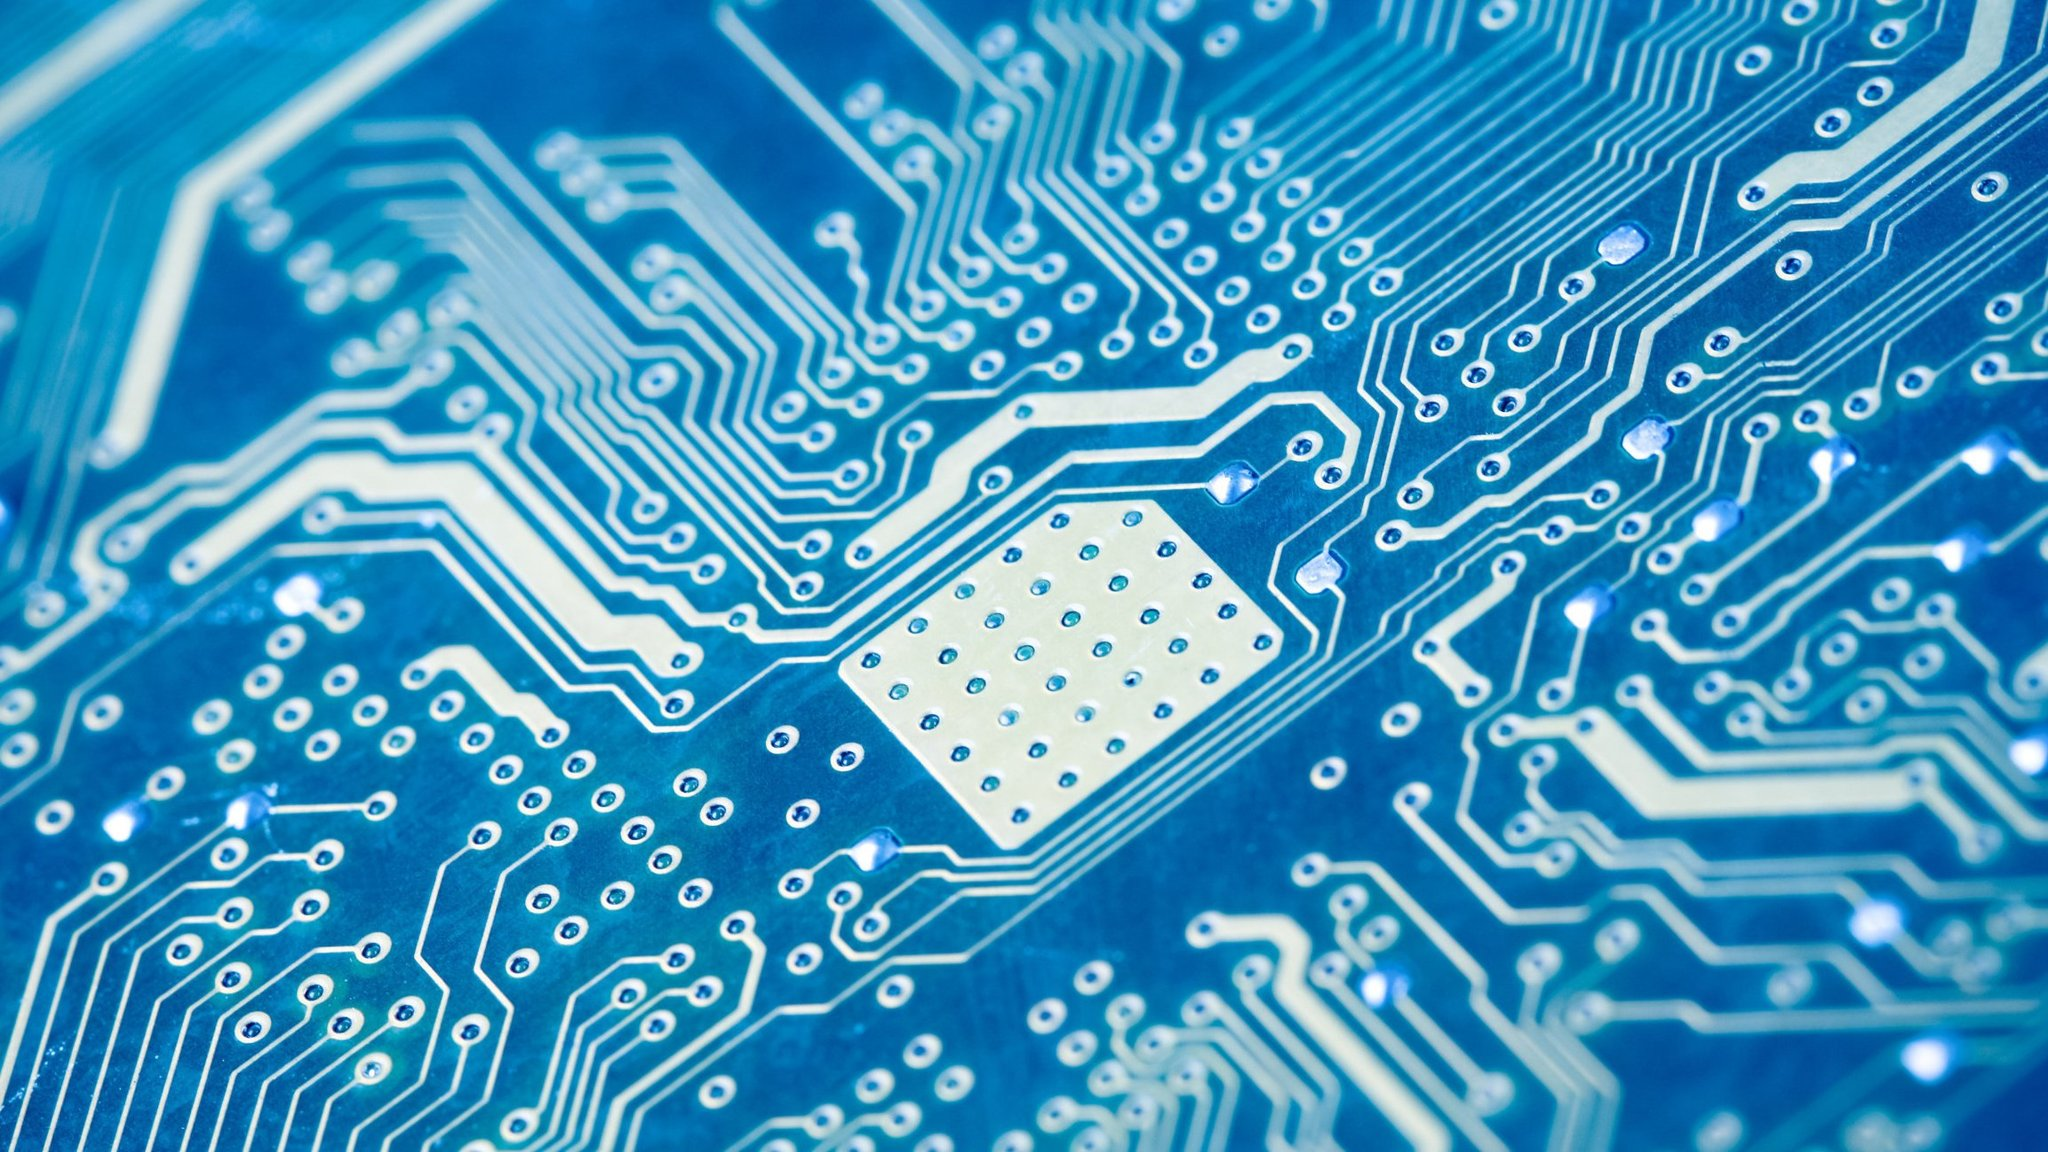
\includegraphics[height=\paperheight,width=\paperwidth]{../03_img/processor.jpg}
			};
		}
		\begin{frame}[plain]
			\vfill
			\begin{boxBlue}
				\centering
				\textbf{Section:} \\
				\large \highlight{#1}
			\end{boxBlue}
			\vfill
			\centering
			
\includegraphics[scale=0.05]{../03_img/logo_dhbw.png}
			\vfill
		\end{frame}
	}
}

% overview page
\newcommand{\makeoverview}[1]{
	\begin{frame}{Lecture Overview}{}
		\begin{tabbing}
			\hspace*{3.5cm}\= \kill
			\ifnum #1=1 \highlight{\textbf{Unit I:}} \else \textbf{Unit I:} \fi
			\> \ifnum #1=1 \highlight{Machine Learning Introduction} \else Machine Learning Introduction \fi \\
		\end{tabbing}
	\end{frame}
}

% thank you page
\newcommand{\makethanks}{
	{\beamertemplatenavigationsymbolsempty
	\begin{frame}[plain]
		\vfill
		\begin{boxBlue}
			\centering
			\Large \highlight{Thank you very much for the attention!}
		\end{boxBlue}
		
		\vfill\footnotesize
		\begin{tabbing}
			\hspace*{1.5cm}\= \kill
			\highlight{Topic:} 	\> \inserttitle \\
			\highlight{Date:} 	\> \insertdate
		\end{tabbing}
		
		\vfill
		\highlight{Contact:} \\
		\insertauthor\ (D062271) \\
		\insertinstitute \\
		\href{mailto:daniel.wehner@sap.com}{\linkstyle{daniel.wehner@sap.com}}
		
		\vfill\normalsize
		\begin{center}
			\large\highlight{Do you have any questions?}
		\end{center}
		\vfill
	\end{frame}}
}

% global pfgplots settings
% --------------------------------------------------------------------------------------------------------
\pgfplotsset{
	% allow filtering of data for pgfplots
	discard if/.style 2 args={
        		x filter/.code={
            		\edef\tempa{\thisrow{#1}}
            		\edef\tempb{#2}
            		\ifx\tempa\tempb
                		\def\pgfmathresult{inf}
            		\fi
        		}
    	},
    	discard if not/.style 2 args={
        		x filter/.code={
            		\edef\tempa{\thisrow{#1}}
            		\edef\tempb{#2}
            		\ifx\tempa\tempb
            		\else
                		\def\pgfmathresult{inf}
            		\fi
        		}
    	}
}


% ====================================================
% ====================================================
% PRESENTATION DATA
% ====================================================
% ====================================================

\title[Clustering]{*** Applied Machine Learning Fundamentals *** Clustering}
\institute{SAP\,SE}
\author{M.\,Sc. Daniel Wehner}
\date{Winter term 2019/2020}
\prefix{CL}

% ====================================================
% ====================================================
% BEGIN OF DOCUMENT
% ====================================================
% ====================================================

\begin{document}

% Title frame
%______________________________________________________________________
\maketitlepage


% Lecture Overview
%______________________________________________________________________
\begin{frame}{Lecture Overview}{}
	\makeoverview{9}
\end{frame}


% Agenda
%______________________________________________________________________
\begin{frame}{Agenda for this Unit}
	\begin{multicols}{2}
		\tableofcontents
	\end{multicols}
\end{frame}


% Section: Introduction
%______________________________________________________________________
\section{Introduction}
\makedivider{Introduction}

% Subsection: What is Clustering?
% --------------------------------------------------------------------------------------------------------
\subsection{What is Clustering?}

% Clustering Introduction
\begin{frame}{Clustering Introduction}{}
	\begin{itemize}
		\item \highlight{Clustering} belongs to the category of \textbf{unsupervised learning}
		\item A clustering algorithm tries to \textbf{find structure} in the data
		\item Once the clusters are found, they first have to be interpreted...
		\item ...and can then be used for prediction purposes
	\end{itemize}
	
	\vspace*{3mm}
	\begin{boxBlueNoFrame}
		\footnotesize
		A cluster must be \highlight{internally homogeneous}, but simultaneously \highlight{externally heterogeneous}.
		(Elements of one cluster have to be very similar, but must differ significantly from elements in other clusters.)
	\end{boxBlueNoFrame}
\end{frame}


% Example Use Cases for Clustering
\begin{frame}{Example Use Cases for Clustering}{}
	\begin{itemize}
		\item \textbf{Behavioral segmentation}
		\begin{itemize}
			\item Customer segmentation (e.\,g. \highlight{sinus milieus})
			\item Creating profiles based on activity monitoring
		\end{itemize}
		\item \textbf{Sorting sensor measurements}
		\begin{itemize}
			\item Image grouping
			\item Detection of activity types in motion sensors
		\end{itemize}
		\item \textbf{Inventory categorization}
		\begin{itemize}
			\item Grouping inventory by sales activity
			\item Grouping inventory by manufacturing metrics
		\end{itemize}
		\item Many, many more, ...
	\end{itemize}
\end{frame}


% Subsection: Clustering Strategies Overview
% --------------------------------------------------------------------------------------------------------
\subsection{Clustering Strategies Overview}

% Clustering Strategies
\begin{frame}{Clustering Strategies}{}
	\begin{enumerate}
		\item \highlight{EM-based clustering}, e.\,g.: $k$-Means
		\item \highlight{Hierarchical clustering}, e.\,g.:
		\begin{itemize}
			\item Agglomerative clustering
			\item Divisive clustering
		\end{itemize}
		\item \highlight{Affinity-based clustering}, e.\,g.:
		\begin{itemize}
			\item Spectral clustering
			\item DBSCAN
		\end{itemize}
	\end{enumerate}
\end{frame}


% Section: $k$-Means
%______________________________________________________________________
\section{$k$-Means}
\makedivider{$k$-Means}

% Subsection: Introduction
% --------------------------------------------------------------------------------------------------------
\subsection{Introduction}

% $k$-Means: Procedure
\begin{frame}{$k$-Means: Procedure}{}\important
	\begin{itemize}
		\item The algorithm is an instance of \highlight{vector quantization}
		\begin{itemize}
			\item It represent data points by a single vector (here: \highlight{centroid}) which is close to them
			\item This is useful for \textbf{compression}!
		\end{itemize}
		\item \textbf{How to}: Create $k$ partitions ($\widehat{=}$ clusters) of the data set $\mathcal{D}$, such that
			the sum of squared deviations from the cluster centroids is \textbf{minimal}:
		\begin{equation}
			\min_{\bm{\mu}_j} \sum_{j=1}^k \sum_{\bm{x}^{(i)} \in \mathcal{D}_j} \Vert \bm{x}^{(i)} - \bm{\mu}_j \Vert^2
		\end{equation}
		\item With $\mathcal{D}_j \equiv j^{th}$ cluster, $\mu_j \equiv$ centroid of $j^{th}$ cluster
	\end{itemize}
\end{frame}


% Result: Voronoi Diagram
\begin{frame}{Result: Voronoi Diagram}{}\important
	\divideTwo{0.49}{
		\begin{itemize}
			\item The dots represent cluster centroids
			\item The lines visualize the \textbf{cluster boundaries}
			\item For a new point we can easily determine to which cluster it has to be assigned
		\end{itemize}
	}{0.49}{
		\begin{figure}
			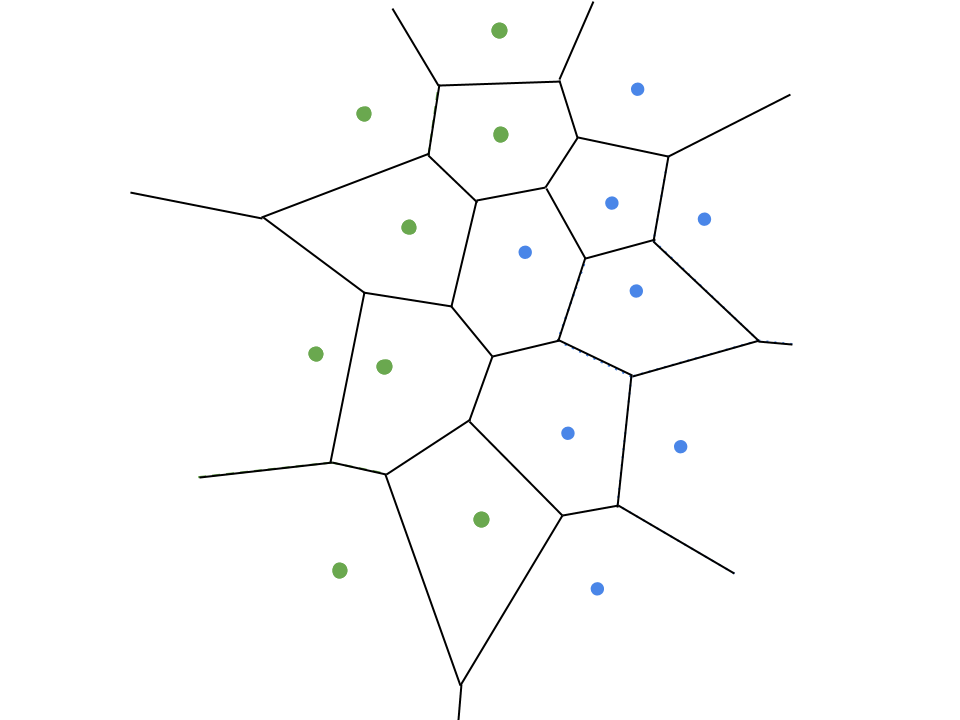
\includegraphics[scale=0.2]{12_clustering/02_img/voronoi}
		\end{figure}
	}
\end{frame}


% Subsection: $k$-Means Algorithm
% --------------------------------------------------------------------------------------------------------
\subsection{$k$-Means Algorithm}

% $k$-Means Algorithm 
\begin{frame}{$k$-Means Algorithm}{}\important
	\vspace*{2mm}
	\begin{itemize}
		\item Input: $\mathcal{D} = \{ \bm{x}^{(1)}, \bm{x}^{(2)}, \dots, \bm{x}^{(n)} \} \in \mathbb{R}^{n \times m}$,
			Number of clusters $k$	
		\item Algorithm:
		\begin{enumerate}
			\item $t \longleftarrow 1$
			\item Randomly choose $k$ means $\bm{\mu}_1^{\langle 1 \rangle}, \bm{\mu}_2^{\langle 1 \rangle}, \dots, \bm{\mu}_k^{\langle 1 \rangle}$ 
			\item While not converged:
			\begin{itemize}
				\item[\textbf{3a}] Assign each $\bm{x}^{(i)} \in \mathcal{D}$ to the closest cluster:
				{\footnotesize
				\begin{equation*}
					\mathcal{D}_j^{\langle t \rangle}
						= \left\{
							\bm{x}^{(i)} : \Vert \bm{x}^{(i)} - \bm{\mu}_j^{\langle t \rangle} \Vert^2 \le
							\Vert \bm{x}^{(i)} - \bm{\mu}_{j^*}^{\langle t \rangle} \Vert^2;\
							\forall j^* = 1, 2, \dots, k; \bm{x}^{(i)} \in \mathcal{D}
						\right\}
				\end{equation*}}
				\item[\textbf{3b}] Update cluster centroids $\bm{\mu}_j$:
				{\footnotesize
				\begin{equation*}
					\bm{\mu}_{j}^{\langle t+1 \rangle} =
						\frac{1}{\vert \mathcal{D}_i^{\langle t \rangle} \vert} \sum_{\bm{x}^{(i)} \in \mathcal{D}_j^{\langle t \rangle}} \bm{x}^{(i)}
					\qquad\text{then update $t$:}\quad t \longleftarrow t + 1
				\end{equation*}}
			\end{itemize}
		\end{enumerate}
	\end{itemize}
\end{frame}


% Subsection: Use Case: Image Compression
% --------------------------------------------------------------------------------------------------------
\subsection{Use Case: Image Compression}

% Image Compression
\begin{frame}{Image Compression}{}
	\begin{figure}
		\centering
		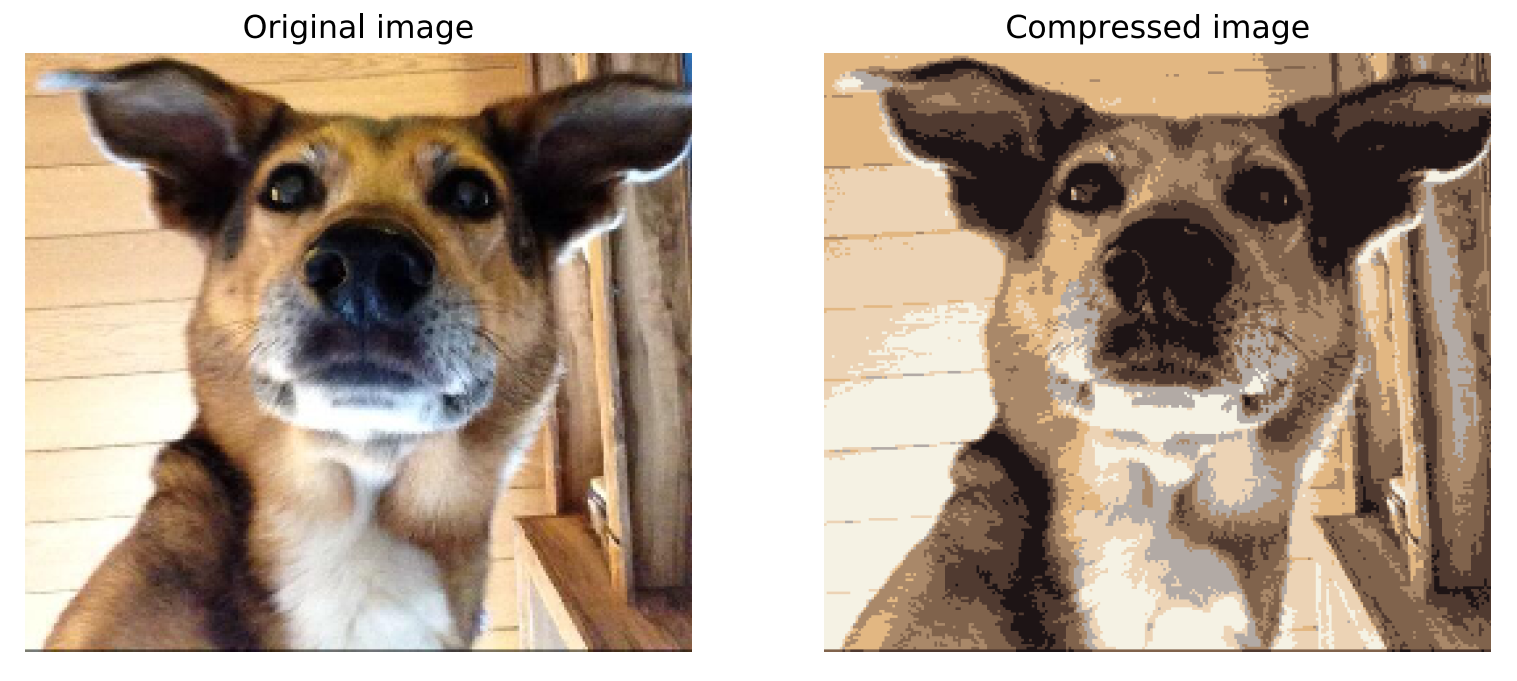
\includegraphics[scale=0.3]{12_clustering/02_img/image_compression}
	\end{figure}
\end{frame}


% Subsection: Problems and Issues
% --------------------------------------------------------------------------------------------------------
\subsection{Problems and Issues}

% $k$-Means Issues
\begin{frame}{$k$-Means Issues}{}
	\begin{itemize}
		\item The algorithm assumes all clusters are \textbf{spherical} \\
			($\ne$ \highlight{affinity-based clustering})
		\item Does not have a notion of \textbf{outliers} (unlike DBSCAN)
		\item What is the correct value for $k$? $\Rightarrow$ \highlight{Elbow-method:}
		\begin{itemize}
			\item Measure sum of squared distances from data points to cluster centers (inertia)
			\item Record results for different values for $k$ and plot them
			\item Search for the `elbow point'
		\end{itemize}
	\end{itemize}
\end{frame}


% Elbow Method
\begin{frame}{Elbow Method}{}
	\begin{figure}
		\centering
		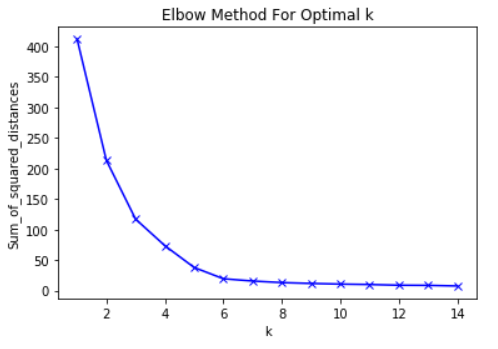
\includegraphics[scale=0.6]{12_clustering/02_img/elbow}
	\end{figure}
\end{frame}


% Section: Hierarchical Clustering
%______________________________________________________________________
\section{Hierarchical Clustering}
\makedivider{Hierarchical Clustering}

% Subsection: Agglomerative Clustering Algorithm
% --------------------------------------------------------------------------------------------------------
\subsection{Agglomerative Clustering Algorithm}

% Agglomerative Clustering Algorithm
\begin{frame}{Agglomerative Clustering Algorithm}{}\important
	\begin{enumerate}
		\item Start with one cluster for each instance: $C = \{ \{ \bm{x}^{(i)}\} : \bm{x}^{(i)} \in \bm{X} \}$
		\item Compute distance $d(C_i, C_j)$ between all pairs of clusters $C_i$, $C_j$
		\item Join clusters $C_i$ and $C_j$ with minimum distance into a new cluster $C_p$:
		\begin{align*}
			C_p
				&= \{ C_i, C_j \} \\
			C
				&= (C \backslash \{ C_i, C_j \}) \cup \{ C_p \}
		\end{align*}
		\item Compute distances between $C_p$ and all other clusters in $C$
		\item If $\vert C \vert > 1$, goto 3
	\end{enumerate}
\end{frame}


% Subsection: Agglomerative Clustering: Example
% --------------------------------------------------------------------------------------------------------
\subsection{Agglomerative Clustering: Example}

% Agglomerative Clustering: Example
\begin{frame}{Agglomerative Clustering: Example}{}
	\begin{figure}
		\centering
		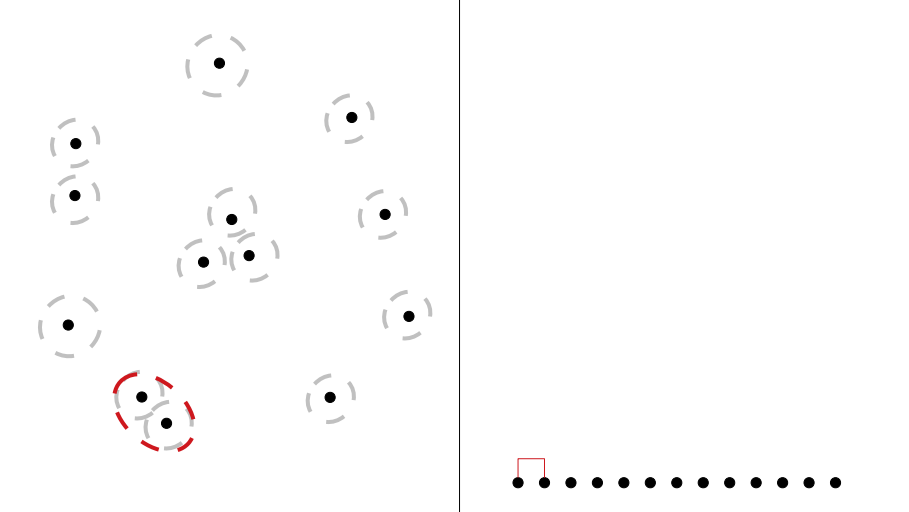
\includegraphics[scale=0.4]{12_clustering/02_img/aggl_clust_1}
	\end{figure}
\end{frame}


% Agglomerative Clustering: Example (Ctd.)
\begin{frame}{Agglomerative Clustering: Example (Ctd.)}{}
	\begin{figure}
		\centering
		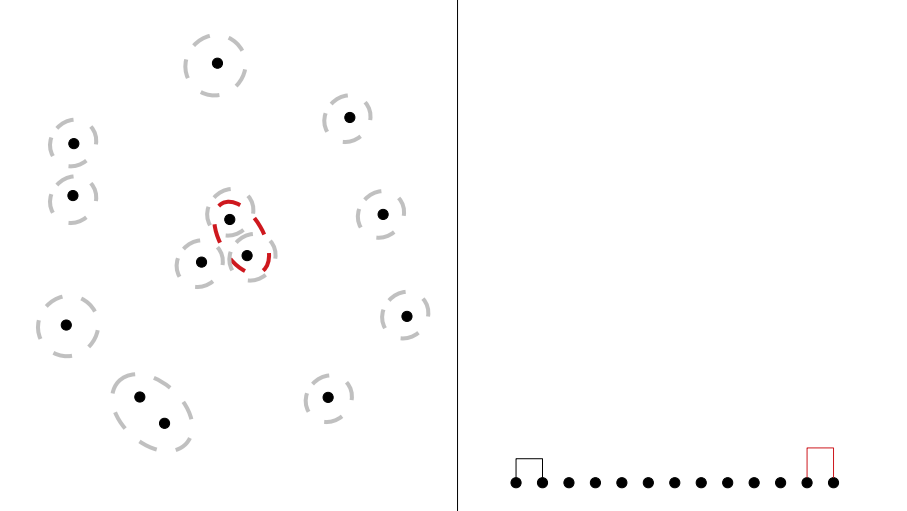
\includegraphics[scale=0.4]{12_clustering/02_img/aggl_clust_2}
	\end{figure}
\end{frame}


% Agglomerative Clustering: Example (Ctd.)
\begin{frame}{Agglomerative Clustering: Example (Ctd.)}{}
	\begin{figure}
		\centering
		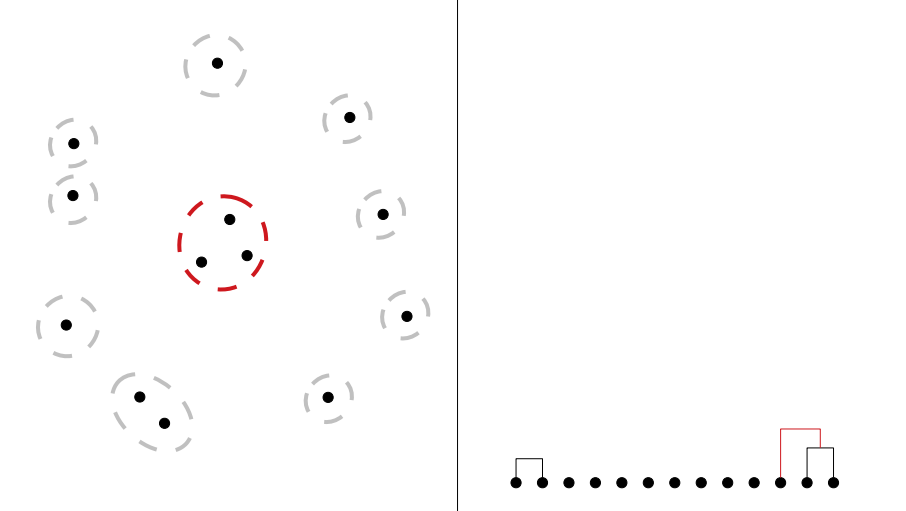
\includegraphics[scale=0.4]{12_clustering/02_img/aggl_clust_3}
	\end{figure}
\end{frame}


% Agglomerative Clustering: Example (Ctd.)
\begin{frame}{Agglomerative Clustering: Example (Ctd.)}{}
	\begin{figure}
		\centering
		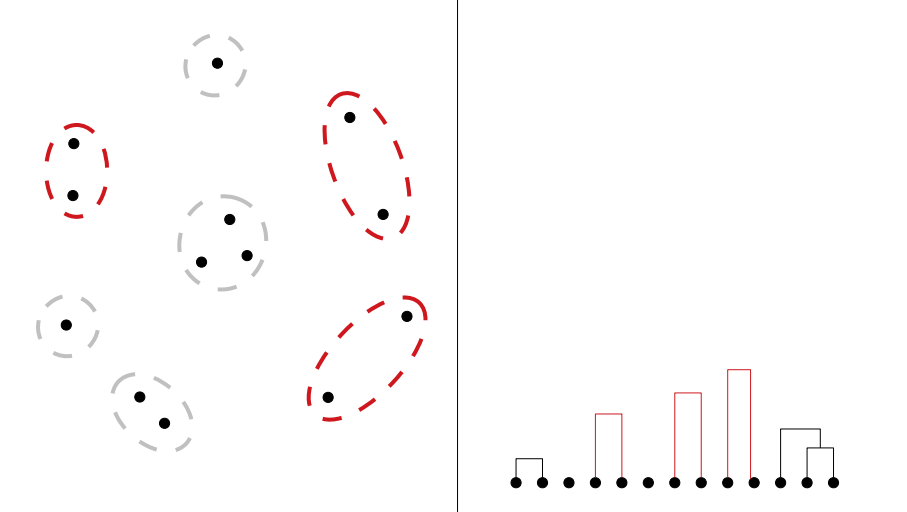
\includegraphics[scale=0.4]{12_clustering/02_img/aggl_clust_4}
	\end{figure}
\end{frame}


% Agglomerative Clustering: Example (Ctd.)
\begin{frame}{Agglomerative Clustering: Example (Ctd.)}{}
	\begin{figure}
		\centering
		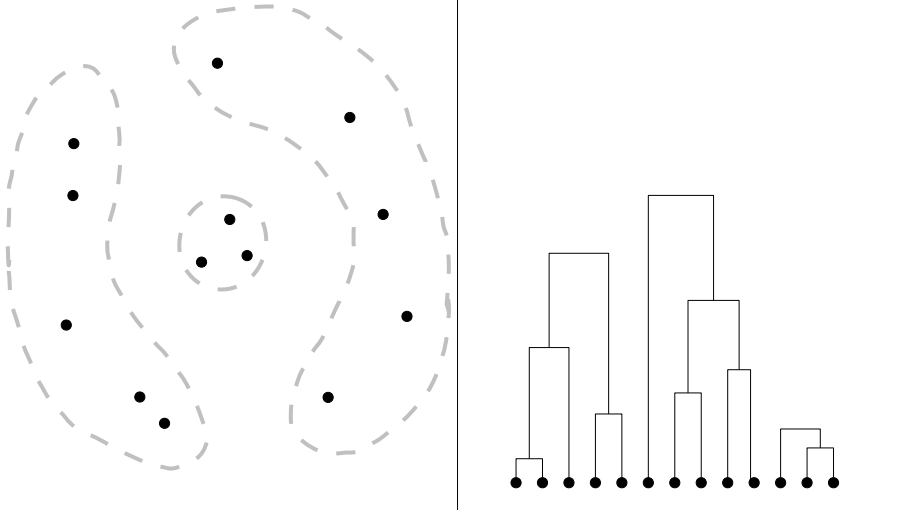
\includegraphics[scale=0.4]{12_clustering/02_img/aggl_clust_5}
	\end{figure}
\end{frame}


% Agglomerative Clustering: Example (Ctd.)
\begin{frame}{Agglomerative Clustering: Example (Ctd.)}{}
	\bubble{13}{5}{
		\footnotesize This is a \\[-2mm]
		\footnotesize \highlight{dendrogram}
	}
	\begin{figure}
		\centering
		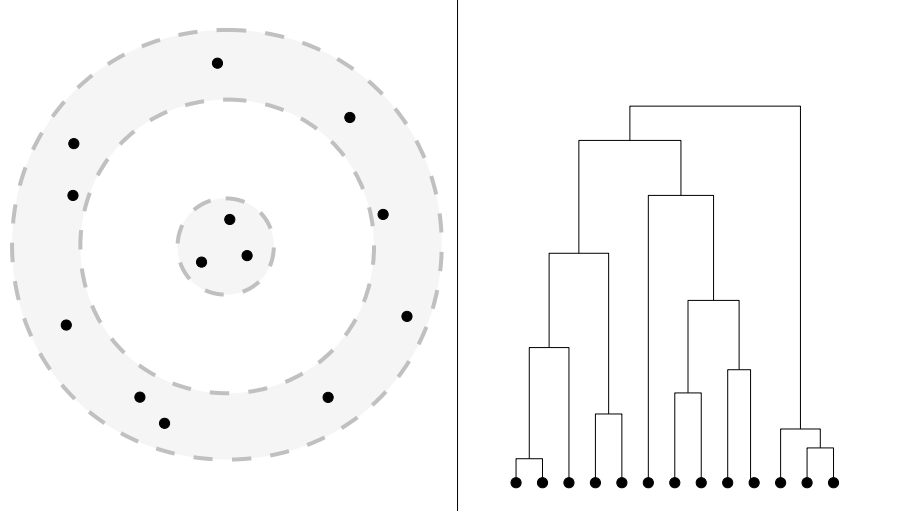
\includegraphics[scale=0.4]{12_clustering/02_img/aggl_clust_6}
	\end{figure}
\end{frame}


% Subsection: Distance Metrics between Clusters
% --------------------------------------------------------------------------------------------------------
\subsection{Distance Metrics between Clusters}

% Single Linkage
\begin{frame}{Single Linkage}{}
	\begin{itemize}
		\item Computing distances between clusters $C_1$ and $C_2$
		\item \highlight{Single linkage}:
		\begin{equation*}
			d(C_1, C_2) = \min\{ d(\bm{x}^{(i)}, \bm{x}^{(j)}) : \bm{x}^{(i)} \in C_1, \bm{x}^{(j)} \in C_2 \}
		\end{equation*}
	\end{itemize}

	\begin{figure}
		\centering
		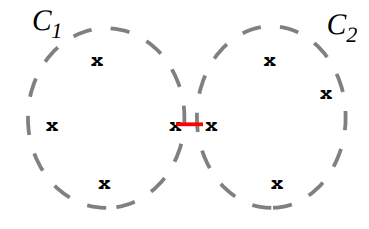
\includegraphics[scale=0.4]{12_clustering/02_img/single_linkage}
	\end{figure}
\end{frame}


% Complete Linkage
\begin{frame}{Complete Linkage}{}
	\begin{itemize}
		\item Computing distances between clusters $C_1$ and $C_2$
		\item \highlight{Complete linkage}:
		\begin{equation*}
			d(C_1, C_2) = \max\{ d(\bm{x}^{(i)}, \bm{x}^{(j)}) : \bm{x}^{(i)} \in C_1, \bm{x}^{(j)} \in C_2 \}
		\end{equation*}
	\end{itemize}

	\begin{figure}
		\centering
		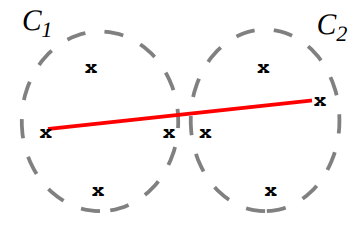
\includegraphics[scale=0.4]{12_clustering/02_img/complete_linkage}
	\end{figure}
\end{frame}


% Section: Spectral Clustering
%______________________________________________________________________
\section{Spectral Clustering}
\makedivider{Spectral Clustering}

% Subsection: Motivation
% --------------------------------------------------------------------------------------------------------
\subsection{Motivation}

% Spectral Clustering
\begin{frame}{Spectral Clustering}{}
	\begin{itemize}
		\item Remember the disadvantage of $k$-Means? (spherical clusters)
		\item How can we cluster data without this assumption?
		\item[$\bm{\Rightarrow}$] \highlight{Affinity-based clustering}
		
		\vspace*{3mm}
		\begin{boxBlueNoFrame}
			\textbf{Affinity-based clustering} assumes \textbf{no shape} of the resulting clusters.
			It is based on the \textbf{connectedness of the data points}.
		\end{boxBlueNoFrame}

		\item Spectral clustering is affinity-based
		\item Whenever you hear \textit{`spectral'}: It has something to do with eigen-vectors
	\end{itemize}
\end{frame}


% Example Data Set
\begin{frame}{Example Data Set}{}
	\bubble{1}{5}{
		\footnotesize What would be \\[-2mm]
		\footnotesize the result of $k$-Means?}
	\begin{figure}
	\centering
	\begin{tikzpicture}[
		scale=0.7
	]

		\begin{axis}[
			xlabel={$\bm{Feature_1}$},
			ylabel={$\bm{Feature_2}$},
			ticks=none,
			x=2cm,
			y=3cm
		]
	
			\addplot[
				only marks,mark=*,mark size=2.5,fill=myblue1
			] table{04_ml_introduction/05_data/data_moons.txt};
    		\end{axis}
	\end{tikzpicture}
\end{figure}
\end{frame}


% Subsection: A Bit of Graph Theory
% --------------------------------------------------------------------------------------------------------
\subsection{A Bit of Graph Theory}

% A short Introduction to Graphs
\begin{frame}{A short Introduction to Graphs}{}
	\begin{itemize}
		\item A graph $\mathcal{G}$ is a tuple $\mathcal{G} = (\mathcal{V}, \mathcal{E})$
		\item $\mathcal{V} = \{ v_1, v_2, \dots, v_n \}$ is the set of $n$ vertices (nodes)
		\item $\mathcal{E} \in \mathcal{V} \times \mathcal{V}$ the set of edges (connections between nodes)
		\item \highlight{Adjacency matrix} $\bm{A}$
		\begin{itemize}
			\item $A_{ij} = 1$, iff $(v_i, v_j) \in \mathcal{E}$ ($v_i$ is a neighbor of $v_j$)
			\item $\bm{A}$ is symmetric for undirected graphs, i.\,e. $A_{ij} = A_{ji}$
		\end{itemize}
		\item The \highlight{degree matrix} $\bm{D} = diag(d_1, d_2, \dots, d_n)$ is a matrix of node degrees
		\begin{equation*}
			d_i = \sum_{j=1}^n A_{ij}
		\end{equation*}
	\end{itemize}
\end{frame}


% A short Introduction to Graphs (Ctd.)
\begin{frame}{A short Introduction to Graphs (Ctd.)}{}
	\begin{itemize}
		\item For graph analysis it is often useful to compute the \highlight{graph Laplacian} matrix:
		\begin{equation*}
			\bm{L} = \bm{D} - \bm{A}
		\end{equation*}
		\item Example:
		\begin{figure}
			\centering
			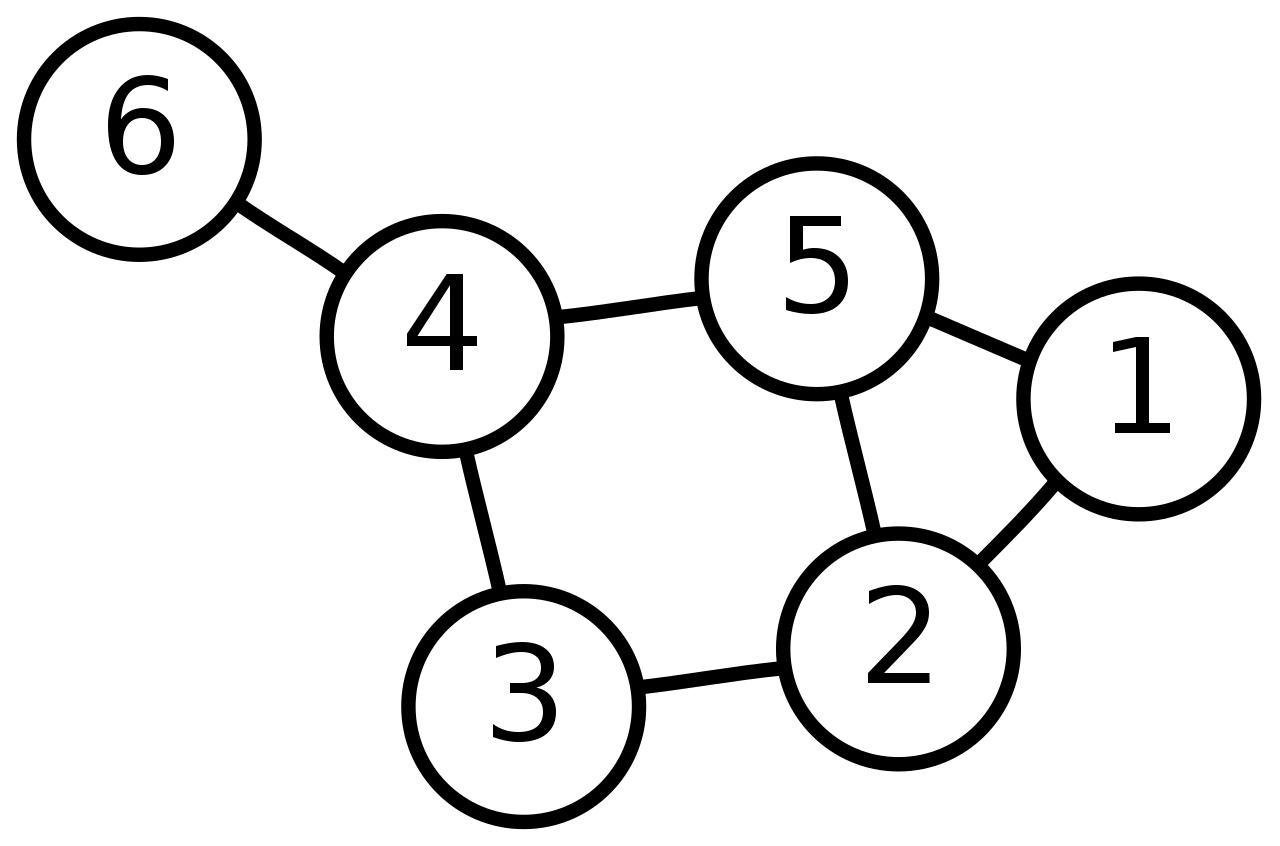
\includegraphics[scale=0.08]{12_clustering/02_img/graph}
		\end{figure}
	\end{itemize}
\end{frame}


% Example: Computation of $\bm{A}$, $\bm{D}$ and $\bm{L}$
\begin{frame}{Example: Computation of $\bm{A}$, $\bm{D}$ and $\bm{L}$}{}
	\scriptsize
	\begin{equation*}
		\bm{A} = \begin{bmatrix}
			0 & 1 & 0 & 0 & 1 & 0 \\
			1 & 0 & 1 & 0 & 1 & 0 \\
			0 & 1 & 0 & 1 & 0 & 0 \\
			0 & 0 & 1 & 0 & 1 & 1 \\
			1 & 1 & 0 & 1 & 0 & 0 \\
			0 & 0 & 0 & 1 & 0 & 0 \\
		\end{bmatrix}\qquad
		\bm{D} = \begin{bmatrix}
			2 & 0 & 0 & 0 & 0 & 0 \\
			0 & 3 & 0 & 0 & 0 & 0 \\
			0 & 0 & 2 & 0 & 0 & 0 \\
			0 & 0 & 0 & 3 & 0 & 0 \\
			0 & 0 & 0 & 0 & 3 & 0 \\
			0 & 0 & 0 & 0 & 0 & 1 \\
		\end{bmatrix}\qquad
		\bm{L} = \begin{bmatrix}
			 \phantom{-}2 	& -1 			& \phantom{-}0 	& \phantom{-}0 	& -1 			& \phantom{-}0 	\\
			-1 			& \phantom{-}3 	& -1 			& \phantom{-}0 	& -1 			& \phantom{-}0 	\\
			 \phantom{-}0 	& -1 			& \phantom{-}2 	& -1 			& \phantom{-}0 	& \phantom{-}0 	\\
			 \phantom{-}0 	& \phantom{-}0 	& -1 			& \phantom{-}3 	& -1 			& -1 			\\
			-1 			& -1 			& \phantom{-}0 	& -1 			& \phantom{-}3 	& \phantom{-}0 	\\
			 \phantom{-}0 	& \phantom{-}0 	& \phantom{-}0 	& -1 			& \phantom{-}0 	& \phantom{-}1 	\\
		\end{bmatrix}
	\end{equation*}
\end{frame}


% Subsection: Spectral Clustering Algorithm
% --------------------------------------------------------------------------------------------------------
\subsection{Spectral Clustering Algorithm}

% How to get the Graph?
\begin{frame}{How to get the Graph?}{}\important
	\begin{itemize}
		\item There are at least two possibilities
		\begin{enumerate}
			\item \highlight{$\varepsilon$-neighborhood graph}
			\begin{itemize}
				\item Connect all instances whose pairwise distances are smaller than $\varepsilon$
				\item \Highlight{Problem:} How to choose $\varepsilon$?
			\end{itemize}
			\item \highlight{$k$-nearest neighbor graph}
			\begin{itemize}
				\item Connect instance $\bm{x}^{(i)}$ with instance $\bm{x}^{(j)}$, if $\bm{x}^{(j)}$ is among the $k$ nearest neighbors of $\bm{x}^{(i)}$
				\item Attention: This definition leads to a directed graph \textbf{(Why?)} \\
					$\Rightarrow$ Can be ignored
				\item \Highlight{Problem:} How to choose $k$?
			\end{itemize}
		\end{enumerate}
		\item Both approaches are used in practice
	\end{itemize}
\end{frame}


% Spectral Clustering Algorithm
\begin{frame}{Spectral Clustering Algorithm}{}\important
	\begin{itemize}
		\item Input: $\mathcal{D} = \{ \bm{x}^{(1)}, \bm{x}^{(2)}, \dots, \bm{x}^{(n)} \} \in \mathbb{R}^{n \times m}$,
			Number of clusters $k$
		\item Algorithm:
		\begin{enumerate}
			\item Construct a similarity graph (adjacency matrix $\bm{A}$ and degree matrix $\bm{D}$)
			\item Compute the graph Laplacian matrix $\bm{L} = \bm{D} - \bm{A}$
			\item Perform \textbf{eigen-decomposition} on $\bm{L}$ (to obtain the eigen-vectors $\bm{Q}$)
			\begin{equation*}
				\bm{L} = \bm{Q}\bm{\Lambda}\bm{Q}^{-1}
			\end{equation*}
			\item Apply $k$-Means to the rows of matrix $\bm{Q}$ to obtain the clusters $\{ C_1, C_2, \dots, C_k \}$
		\end{enumerate} 
	\end{itemize}
\end{frame}


% Section: Wrap-Up
%______________________________________________________________________
\section{Wrap-Up}
\makedivider{Wrap-Up}

% Subsection: Summary
% --------------------------------------------------------------------------------------------------------
\subsection{Summary}

% Summary
\begin{frame}{Summary}{}
	\begin{itemize}
		\item Clustering belongs to the category of \textbf{unsupervised learning}
		\item With clustering we try to find \textbf{structure in the data}
		\item Different algorithms make \textbf{different assumptions} about the resulting clusters
		\item \textbf{Clustering Strategies:}
		\begin{itemize}
			\item EM-based clustering (e.\,g. $k$-Means)
			\item Affinity-based clustering (e.\,g. spectral clustering, DBSCAN)
			\item Hierarchical clustering
		\end{itemize}
	\end{itemize}
\end{frame}


% Subsection: Self-Test Questions
% --------------------------------------------------------------------------------------------------------
\subsection{Self-Test Questions}

% Self-Test Questions
\begin{frame}{Self-Test Questions}{}\important
	\begin{enumerate}
		\item What is clustering?
		\item What is the definition of a cluster. Which properties should it have?
		\item Describe the general procedure of $k$-Means. What are disadvantages?
		\item What is a dendrogram?
		\item How do we obtain the graphs for spectral clustering
		\item What is affinity-based clustering. How does it differ from $k$-Means?
		\item How to calculate the graph Laplacian matrix?
	\end{enumerate}
\end{frame}


% Subsection: Lecture Outlook
% --------------------------------------------------------------------------------------------------------
\subsection{Lecture Outlook}

\begin{frame}{What's next...?}{}
	\makeoverview{10}
\end{frame}


% Subsection: Recommended Literature and further Reading
% --------------------------------------------------------------------------------------------------------
\subsection{Recommended Literature and further Reading}

% Literature
%______________________________________________________________________
\begin{frame}[allowframebreaks]{Recommended Literature and further Reading}{}
	\footnotesize
	\begin{thebibliography}{2}
		\literature{book}{Bishop.2006}{[1] Pattern Recognition and Machine Learning}
			{Christopher Bishop. Springer. 2006.}{$\rightarrow$ \href{
				http://users.isr.ist.utl.pt/~wurmd/Livros/school/Bishop\%20-\%20Pattern\%20Recognition\%20And\%20Machine\%20Learning\%20-\%20Springer\%20\%202006.pdf
			}{\linkstyle{Link}}, cf. chapter 9}
		\literature{book}{Murphy.2012}{[2] Machine Learning: A Probabilistic Perspective}
			{Kevin Murphy. MIT Press. 2012.}{$\rightarrow$ \href{
				https://doc.lagout.org/science/Artificial\%20Intelligence/Machine\%20learning/Machine\%20Learning_\%20A\%20Probabilistic\%20Perspective\%20\%5BMurphy\%202012-08-24\%5D.pdf
			}{\linkstyle{Link}}, cf. chapter 25}	
	\end{thebibliography}
\end{frame}


% Subsection: Meme of the Day
% --------------------------------------------------------------------------------------------------------
\subsection{Meme of the Day}

% Meme of the Day
\begin{frame}{Meme of the Day}{}
	\begin{figure}
		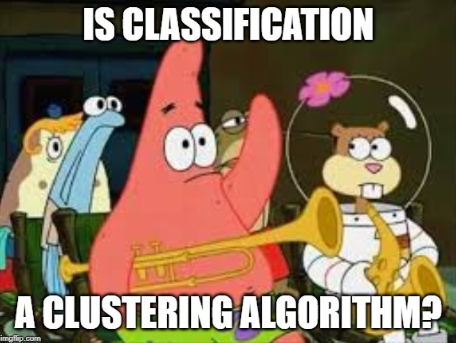
\includegraphics[scale=0.5]{12_clustering/02_img/meme_of_the_day}
	\end{figure}
\end{frame}


% Thank you
%______________________________________________________________________
\makethanks

\end{document}